\documentclass[12pt,letterpaper,noanswers]{exam}
\usepackage[usenames,dvipsnames,svgnames,table]{xcolor}
\usepackage[margin=0.9in]{geometry}
\renewcommand{\familydefault}{\sfdefault}
\usepackage{multicol}
\usepackage{wrapfig}
\pagestyle{head}
\definecolor{c03}{HTML}{FFDDDD}
\header{AM 22b Class 09}{}{Feb 17: chain rule, directional derivative}
\runningheadrule
\headrule
\usepackage{graphicx} % more modern
\usepackage{amsmath} 
\usepackage{amssymb} 
\usepackage{hyperref}
\usepackage{tcolorbox}

\usepackage[numbered,autolinebreaks,useliterate]{mcode}

\newcommand{\mb}[1]{\underline{#1}}

\begin{document}
 \pdfpageheight 11in 
  \pdfpagewidth 8.5in




% I need to review the torus trajectories...

\begin{itemize}
% \item There is a pre-class assignment (20 minutes of videos + a few WeBWorK exercises) due at 10am this Monday.  It is available on Canvas.
\itemsep0em
    % \item PSet 02 is due on Friday Feb 14th at 10am.
    \item There is a quiz on Friday (available until Sunday at 6pm ET).  It is self-scheduled, will be administered via Gradescope, and will last 60 minutes (you'll have 75 minutes of access time).  The topic info is on Canvas.
    \item There is a skill check in class on Monday.  The sample problem are in the C08, C09, C10 handouts.
\end{itemize}

\hrule
\vspace{0.2cm}

% partial derivatives, gradient
% local linearity, differential, directional deriv
% 2nd order partials + equations with partials

\noindent\textbf{Big picture}

This week we are studying differentiation.  Today our focus is on rates of change in the case of function composition (chain rule).

\vspace{0.2cm}
\hrule
\vspace{0.2cm}


\noindent\textbf{Teams}

\begin{multicols}{2}

\noindent 1. If you'd like to work alone today, go to breakout room 1.

\noindent 2. If you'd like to work in a team, go to breakout room 2, and Sarah will assign you to a team.

\end{multicols}

%\vspace{0.2cm}
\hrule
\vspace{0.2cm}

\noindent\textbf{Skill Check C09 practice}

\begin{questions}
\item Compute the directional derivative of $f(x,y) = 3x^2y$ at $(1,0)$ in the direction of $\mb{u} = \langle 1,3\rangle$.
\item Find the maximum possible directional derivative at $(1,0)$ (choosing from any direction).
\end{questions}

\vspace{0.2cm}
\hrule
\vspace{0.2cm}

\noindent\textbf{Skill Check C09 practice solution}

$Df = [6xy, 3x^2]$.  At $(1,0)$ this is $[0, 3]$.  Creating a unit vector in the direction of interest, $\hat{\mb{u}}=\mb{u}/\Vert\mb{u}\Vert = \left(\begin{array}{c} 1/\sqrt{10} \\ 3/\sqrt{10}\end{array}\right)$.

The directional derivative is $f_{\mb{u}} =[0, 3]\left(\begin{array}{c} 1/\sqrt{10} \\ 3/\sqrt{10}\end{array}\right) = 0(1/\sqrt{10}) + 3(3/\sqrt{10}) = 9/\sqrt{10}$.

The maximum possible directional derivative is $\Vert \nabla f \Vert = \Vert Df \Vert = 3.$

\vspace{0.2cm}
\hrule
\vspace{0.2cm}



\noindent\textbf{Single variable chain rule}
\begin{tcolorbox}
Let $y = y(x)$ and $x = x(t)$.  The \textbf{chain rule} states that $\left.\frac{dy}{dt}\right\vert_{t=a} = \left.\frac{dy}{dx}\right\vert_{x=x(a)}\left.\frac{dx}{dt}\right\vert_{t=a}.$

In other notation, let $f:\mathbb{R}\rightarrow\mathbb{R}$ and $g:\mathbb{R}\rightarrow\mathbb{R}$.  $\left.(f\circ g)'(x)\right\vert_{x=a} = \left.f'(g(x))\right\vert_{g(x)=g(a)}\left.g'(x)\right\vert_{x=a}$
\end{tcolorbox}

I think of the chain rule as 
encoding the idea that sensitivity of $y$ to change in $t$ exists because $y$ depends on $x$ and $x$ is sensitive to change in $t$.

\noindent\textbf{Examples.}
\begin{enumerate}
\item Let $y(x) = x^3$ and $x(t) = \sin t$.  Find $\left.\frac{dy}{dt}\right\vert_{t=\pi/4}$
\vspace{2cm}

\item Find an expression for $dy$ in terms of $dt$ at $t = \pi/4$.
\vspace{1.5cm}

\item The period, $T$, of oscillations (in seconds) of a pendulum clock is given by $T = 2\pi\sqrt{L/g}$ where $g$ is the acceleration due to gravity.  The length, $L$, of the clock depends on temperature, $h$, by expanding when it is warm. $L \approx L_0(1+ \alpha(h-h_0))$.  Find an expression for $\Delta T$ in terms of $\Delta h$, where we center the approximations at $h = h_0, L = L_0, T = 2\pi\sqrt{L_0/g}$.
\vspace{3cm}

\end{enumerate}

\noindent\textbf{Chain rule} \S 14.6
\begin{tcolorbox}
\begin{itemize}
\itemsep0em
    \item For differentiable functions $\mb{f}$ and $\mb{g}$, let $\mb{f}: \mathbb{R}^m \rightarrow \mathbb{R}^p$ and $\mb{g}: \mathbb{R}^n\rightarrow\mathbb{R}^m$.  The composition is $\mb{f} \circ \mb{g}: \mathbb{R}^n\rightarrow\mathbb{R}^p$. \emph{(Rates of change multiply under composition.)}
    
    The \textbf{multivariable chain rule} states that $[D \mb f\circ \mb g]_{\mb{a}} = [D\mb f]_{\mb{g}(\mb{a})}[D\mb g]_{\mb{a}}$.
    
\item This can also be written in Leibniz notation.  Let $\mb{y} = \mb{y}(\mb{x})$ and $\mb{x} = \mb{x}(\mb{u})$.  We have    
    $\displaystyle\left.\frac{\partial\mb{y}}{\partial\mb{u}}\right\vert_{\mb{u}=\mb{a}}~=~\left.\frac{\partial\mb{y}}{\partial\mb{x}}\right\vert_{\mb{x}=\mb{x}(\mb{a})}\left.\frac{\partial\mb{x}}{\partial\mb{u}}\right\vert_{\mb{u}=\mb{a}}$.  
    \item \emph{Notice that $\frac{\partial\mb{y}}{\partial\mb{u}}$ and $\frac{\partial\mb{x}}{\partial\mb{u}}$ are evaluated at $\mb{u} = \mb{a}$ while $\frac{\partial\mb{y}}{\partial\mb{x}}$ is evaluated at $\mb{x} = \mb{x}(\mb{a})$.}
    \item We sometimes use $\mb{y}(\mb{u})$ to denote $\mb{y}(\mb{x}(\mb{u}))$.
    \end{itemize}
    \end{tcolorbox}
    
    \noindent\textbf{Example}. Given $f(x,y) = \left(\begin{array}{c} x^2+y^2 \\ xy \end{array}\right)$ and $g(u,v) = \left(\begin{array}{c} 2u - v \\ v-u \end{array}\right)$ and the outputs of $(f \circ g)$ at $u=1, v=2$ change at a rate of $\left(\begin{array}{c} -4 \\ 3 \end{array}\right)$.  Find the rates of change of the inputs $u, v$.  \emph{Note: as a first step, figure out the values of $x$ and $y$ that are relevant for this problem.}
    
    \vspace{2.5in}
    
    \eject
    
    \noindent\textbf{Example}.  A bison is moving around and is at location $(x,y)$ at time $t$.  The temperature, $H$, near the bison is given by $H = f(x,y,t)$.  North is in the direction of increasing $y$ and the temperature changes with latitude.  There is a cold front coming from the east, and the sun is heating the air as time passes from sunrise.  
 
 Let $\underline{u} = (x,y,t)^T$.
 
 $\displaystyle\frac{dH}{dt} = \frac{\partial H}{\partial\mb{u}}\frac{\partial\mb{u}}{\partial t} = \left[\frac{\partial f}{\partial x}, \frac{\partial f}{\partial y}, \frac{\partial f}{\partial t}\right]\left(\begin{array}{c} \frac{dx}{dt} \\ \frac{dy}{dt} \\ 1 \end{array}\right) = \frac{\partial f}{\partial x}\frac{dx}{dt} + \frac{\partial f}{\partial y}\frac{dy}{dt} + \frac{\partial f}{\partial t}$.
 
 The bison is experiencing an instantaneous rate of change of temperature due to 
 \begin{enumerate}
     \item the rising sun
     \item the coming cold front
     \item the bison's change in latitude
 \end{enumerate}
 
 Match each of these to one of the terms in the chain rule expression.
 \vspace{1in}
    
    \begin{tcolorbox}
    \begin{itemize}
        \itemsep0em
    \item Consider the scalar valued function $f(x,t)$ where $x$ is itself a function of $t$.  The \textbf{total derivative} $\displaystyle\frac{df}{dt}$ is $\displaystyle\frac{df}{dt} = \frac{\partial f}{\partial x}\frac{dx}{dt} + \frac{\partial f}{\partial t}$.
    \item We will follow the convention that $\displaystyle\frac{\partial f}{\partial t}$ indicates the result of differentiating $f$ with respect to the explicitly appearing variable $t$, holding all other explicitly appearing variables (here $x$) constant.  Another way to denote that is $\displaystyle\left(\frac{\partial f}{\partial t}\right)_x$.
    \item Consider the function $z = f(x,y,t)$ where $x$ and $y$ are functions of $t$ and $s$.  In this case we must use the explicit convention above: $\displaystyle\left(\frac{\partial f}{\partial t}\right)_s = \frac{\partial f}{\partial x}\frac{\partial x}{\partial t} + \frac{\partial f}{\partial y}\frac{\partial y}{\partial t} + \frac{\partial f}{\partial t}$.
\end{itemize}


\end{tcolorbox}



\vspace{0.2cm}
\hrule
\vspace{0.2cm}


\noindent\textbf{Directional derivative} \S 14.4-14.5

\begin{tcolorbox}
\begin{itemize}
\itemsep0em
    \item This is a common term in classical vector calculus.
    \item If you have a scalar valued function $f$, and want to compute a derivative of $f(\mb{x})$ 'along a direction' $\mb{u}$, you create a unit vector in the direction of interest and apply the linear transformation $Df$ to $\hat{\mb{u}} = \dfrac{\mb{u}}{\Vert\mb{u}\Vert}$, $[D\mb{f}]\hat{\mb{u}}$.  It is often written $\nabla \mb{f} \cdot \hat{\mb{u}}.$
    \item Our text will denote this 'directional derivative' as $\left.f_{\mb{ u}}\right\vert_{(a,b)}$.
    \item We can apply the linear transformation $D\mb{f}$ to any vector of rates of change, $\mb{h}$, $[D\mb{f}]\mb{h}$, to learn about the sensitivity of $\mb{f}$, so the directional derivative is a limited special case.  It only makes sense when all of the inputs to $f$ have the same units.
\end{itemize}
\end{tcolorbox}

\noindent\textbf{Worked Example}

Let $f(x,y) = 3x^2+y^2$.  Consider the cross-section of the graph of the function that is given by $y = 2x + 1$.  Find the slope of the tangent line to $f(x,y)$ in that cross section, when $x = -0.5$ and $x$ is increasing.  

\emph{This slope is the directional derivative of $f$.  The direction is set by moving along the cross-section in the $xy$-plane such that $x$ is increasing}.

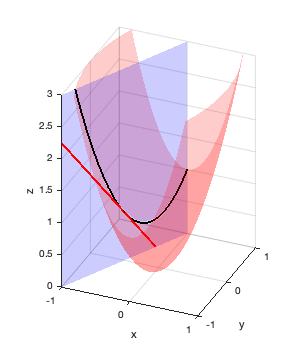
\includegraphics[scale=0.5]{img/C09tangent.png}
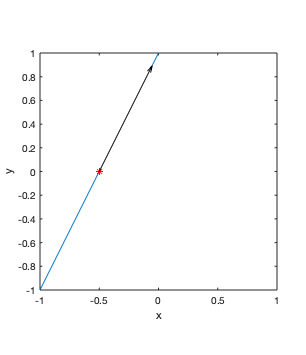
\includegraphics[scale=0.5]{img/C09tangentxy.png}

\begin{itemize}
\itemsep0em
    \item The directional derivative requires a point and a vector in the domain of $f(x,y)$.  (See plot on the right).
    \item The point is at $(x,y) = (-0.5, 2(-0.5)+1) = (-0.5,0)$.
    \item To find the vector direction, we have $y = 2x+1$ so $\Delta y = 2\Delta x$ and $\mb{u} = \langle 1, 2\rangle$.  The corresponding unit vector is $\hat{\mb{u}} = \mb{u}/\sqrt{5}$.
    \item $Df = (6x, 2y)$. $\left.Df\right\vert_{(-0.5,0)} = (-3,0)$
    \item The directional derivative is $\left.Df\right\vert_{(-0.5,0)} \hat{\mb{u}} = (-3,0)\left(\begin{array}{c} 1/\sqrt{5} \\ 2/\sqrt{5} \end{array}\right) = -3/\sqrt{5}$
\end{itemize}

The slope of the red line in the figure above is given by $-3/\sqrt{5}$.  For each unit of motion along the line $y = 2x+1$ in $xy$-space (with $x$ increasing), the $z$ value of the line moves down by $-3/\sqrt{5}$.



\noindent\textbf{Example}

 Let $f(x,y,z)$ represent the temperature in degrees C at the point $(x,y,z)$ with $x,y,z$ in meters.  Assume you are moving at $\mb{v}$ meters per second through space.

The instantaneous rate of change of your temperature with respect to time is given by $[Df] \mb{v} = f_{\mb{v}}\Vert \mb{v}\Vert.$

Identify the dimensions or units for each of $\Vert \mb{\nabla} f\Vert$, $f_{\mb{v}}$, $\mb{\nabla} f\cdot \mb{v}$, $\mb{\nabla} f\cdot \hat{\mb{v}}$.
\vspace{1in}


\item Let $f(x,y) = 3x^2+y^2$.  Construct a tangent plane to the graph of function about the point $(-1,1,4)$.


\begin{tcolorbox}
\begin{itemize}
    \item The \textbf{directional derivative} is sometimes described as the instantaneous rate of change of the function along the direction of $\mb{u}$ (where $\mb{u}$ is a vector in the domain of the function).
    \item Using the geometric definition of the dot product, $\left.f_{\mb{ u}}\right\vert_{(a,b)} = \left.Df\right\vert_{(a,b)}\hat{\mb{u}} = \left.\mb{\nabla}f\right\vert_{(a,b)}\cdot \hat{\mb{u}} = \Vert \mb{\nabla}f\Vert{(a,b)}\Vert\hat{\mb{u}}\Vert\cos\theta = \Vert \mb{\nabla}f\Vert_{(a,b)}\cos\theta$.
    \item At a point $(a,b)$, the directional derivative \textbf{has a maximum} (over all possible directions) $\Vert \mb{\nabla}f\Vert_{(a,b)}$ and a minimum of $-\Vert \mb{\nabla}f\Vert_{(a,b)}$.  The maximum occurs when $\mb{u}$ is a positive scalar multiple of $ \left.\mb{\nabla}f\right\vert_{(a,b)}$.
\end{itemize}
\end{tcolorbox}







\end{document}